\chapter{Event Selection}
\label{chap:eventselection}

\section{Analysis Strategy}

This analysis aims to select events that would have small cross sections producing only a handful of events from the entire 139 \ifb collected by \ac{ATLAS}. The signature of two displaced leptons, is rather simple in principle, but this analysis had not been done before in the conditions of the \ac{LHC}, so extensive optimization of the signal regions and lepton selection criteria needed to be done. A cut in the event selection should decrease or eliminate some background, but have little to no impact on the signal. For example, quality criteria ensure that leptons are well measured in the detector, and leptons from slepton decays will pass these quality criteria, but fake leptons from reconstruction failures generally will not. Every effort was made to remain as signal-agnostic as possible, so cuts on the specific topology of the \ac{GMSB} \ac{SUSY} decay were avoided. 

This analysis is split into three signal regions, defined by the flavor of the two highest \pt leptons in the event: SR-$ee$ with two electrons, SR-$\mu\mu$ with two muons, and SR-$e\mu$ with an electron and a muon.
There are two definitions of leptons used: \emph{baseline} and \emph{signal}. Baseline leptons are required to pass the reconstruction and identification criteria described in \autoref{sec:el_reco_mods} and \autoref{sec:mu_reco_mods} and have $\pt > 50 \GeV$ and $\absdz > 2$ mm. Signal muons are required to further pass bespoke quality requirements, an isolation cut, and have $\pt > 65 \GeV$ and $\absdz > 3$ mm. Displacement-independent quality variables, described in the rest of this chapter, were defined specifically for this analysis as many standard quality criteria place requirements on the \absdz, \absz, or the number of hits in the Pixel detector, all of which would limit the ability to target displaced leptons.

\subsection{Background Overview}
The two signal leptons are required to have high \pt and high \absdz, higher than that expected of any leptons resulting from \ac{SM} processes. The remaining backgrounds come from failures of reconstruction algorithms, extreme tails of decays of \acf{HF} physics (b-jets or $\tau$s), and muons from cosmic rays. None of these background sources are well modeled in \ac{MC}, so data-driven methods must be used. This brings additional challenges from statistical limitations and care must be taken to avoid unblinding the signal regions.

Fake leptons result from the mis-association of a track to a calorimeter or \ac{MS} signature, creating a reconstructed lepton that does not correspond to a real particle that passed through the detector. 
This is particularly likely due to use of \ac{LRT}. The extended tracking algorithm loosens several requirements that enable high-\absdz tracking, but also introduces many \emph{fake tracks}, combinations of hits that do not correspond to the trajectory of a particle in the detector. When matched to \ac{MS} or calorimeter signatures, high-\absdz leptons can be created and form a background to this search. This is particularly likely to occur during electron reconstruction, where the track can be associated to real calorimeter signatures from photons or converted photons. 

The background to SR-$\mu\mu$ is dominated by cosmic ray muons. The \ac{ATLAS} detector is far underground partially to avoid the many particles from cosmic rays passing through the detector. However, there is a service shaft above the detector and muons can make it through the earth above the detector, so muons from cosmic rays are constantly passing through the detector. If a muon from a cosmic ray passes through the detector and is coincident with a bunch crossing, the event could be triggered and that muon reconstructed. Since it can pass at any point with respect to the collision, it can be reconstructed as one or two muons with high \absdz, exactly mimicking the targeted signature. 

Both electrons and muons suffer potential backgrounds from \ac{HF} decays, predominately from the decays of b-hadrons. b-quarks are very commonly produced in \ac{LHC} collisions and they immediately hadronize into b-hadrons, which have a lifetime of 1.5 ps and whose decays include a lepton 11\% of the time \cite{pdg}. This is sufficiently long that the b-hadron travels far enough before it decays such that a secondary vertex can be identified. Generally, the tracks have low \pt and maximum \absdz of about 1.5 mm, and the 3 mm cut on signal leptons is designed to minimize this effect. However, it is possible that extreme tails of this distribution are not well modeled in \ac{MC} and in an analysis where 0 background events are expected, understanding each possible source is paramount.


\section{Event Requirements}

Events must pass a trigger in order to be recorded by the \ac{ATLAS} detector. Three different triggers are used in this analysis and the data separated into three orthogonal regions based on the topology of the event, described in \autoref{tab:triggers}. The trigger is required to pass in the appropriate region for the event to be selected.

Each event is required to pass a standard set of \ac{ATLAS} event quality preselection criteria. Specifically, these include detector error flags which reject events with noise bursts or data corruption, or events in periods where any sub-detector was operating suboptimally. Events are required to have at least one \ac{PV} with $|z| < 200$ mm.

From events that pass the previous two requirements, events are sorted into the three signal regions based on the highest \pt baseline leptons in the event. Leptons in signal events are required to be well separated with $\dR_{\ell\ell} > 0.2$. This eliminates background from lepton pairs that could be created from an interaction with the material of the detector. Finally, signal events are required to have zero cosmic muons. The cosmic tag and the associated background will be discussed in \autoref{sec:cosmics}. The analysis was optimized and the backgrounds estimated while keeping the \acp{SR} blinded, so \acp{CR} (where backgrounds are estimated) and \acp{VR} (where additional studies and validation are done) are defined with different numbers of leptons and cosmic tags. All \acp{CR} and \acp{VR} are designed to be dominated by backgrounds and have very few signal events in them. A full list of all signal, control, and validation regions can be seen in \autoref{tab:regions}. 


\begin{sidewaystable}[!ht]
\small
\begin{center}
\begin{tabular}{l|l|c|c|c}
Purpose & Name & \# of Leptons & \# of Cos.Tags & Additional Requirements\\
\hline
%\multicolumn{5}{|c|}{Signal Regions} \\
%\hline
\multirow{3}{*}{Signal Regions} & SR-$ee$ 	& $\geq$ 2 $e$ 						& 0  & \\
								& SR-$\mu\mu$ & $\geq$ 2 $\mu$ 					& 0  & \\
								& SR-$e\mu$ 	& $\geq$ 1 $e$, $\geq$ 1 $\mu$  & 0  & \\
\hline
\multicolumn{5}{c}{Control Regions} \\
\hline
\multirow{2}{*}{Fake Estimation} 	&CR-$ee$-fake		& $\geq$ 2 $e$					& 0		& $\geq$ 2 loosened electrons, not in SR-$ee$  \\
									&CR-$e\mu$-fake		& $\geq$ 1 $e$, $\geq$ 1 $\mu$ 	& 0		& $\geq$ 2 loosened leptons, not in SR-$e\mu$  \\
\hline
Heavy Flavor Estimation 			&CR-$\mu\mu$-hf		& $\geq$ 2 $\mu$				& 0 	& $\geq$ 1 anti-isolated $\ell$, loosened \pt and \dz \\
\hline
\multirow{2}{*}{Cosmic Estimation} 	&CR-$M_{\mathrm{full}}$  & $\geq 1 \mu$		& $\geq 1$ 	    &  includes muons failing \nphi and \nprecision cuts\\
									&CR-$\mu\mu$-topbad	& $\geq$ 2 $\mu$				& 0  	& one signal and one loosened muon \\
\hline
\multicolumn{5}{c}{Validation Regions} \\
\hline
\multirow{4}{*}{Cut Evaluation}		&VR-$M_{\mathrm{narrow}}$& $\geq 1 \mu$		& $\geq 1$ 	& using narrow cosmic tag \\ 
									&VR-$e$					& 1 $e$, 0 $\mu$	& 0 		& electron is baseline  \\
									&VR-$\mu$				& 0 $e$, 1 $\mu$	& 0 		& muon is baseline  \\   
% evaluating cleaning cuts
\hline
\multirow{4}{*}{Fake Validation}	&VR-$ee$-fake			& $\geq$ 2 $e$					& 0 & inverted \dpt selection \\
									&VR-$ee$-fake-hf		& $\geq$ 2 $e$					& 0 & $\geq 1$ anti-isolated $\ell$, loosened quality  \\
									&VR-$e\mu$-fake			& $\geq$ 1 $e$, $\geq$ 1 $\mu$ 	& 0 & 1 $e$ fails \dpt, 1 $\mu$ fails \chiCB \\ 
									&VR-$e\mu$-fake-hf		& $\geq$ 1 $e$, $\geq$ 1 $\mu$	& 0 & 1 $e$ fails \dpt, no isolation req., loosened quality \\
% Validation of fake estimates, including HF contribution
\hline
\multirow{3}{*}{Cosmic Validation}	&VR-$\mu M_{\mathrm{full}}$  & $\geq$ 2 $\mu$			& 1 	& \\		
									&VR-$\mu$-narrow 			& $\geq$ 1 $\mu$			& 0* 	& using narrow cosmic tag \\
									&VR-$\mu M_{\mathrm{narrow}}$& $\geq$ 2 $\mu$			& 1* 	& using narrow cosmic tag \\
% Validation of cosmics

\hline
\end{tabular}
\caption{Summary of signal, control and validation regions used in the analysis. All regions are defined exclusively by their reconstructed leptons. In the table, all leptons should be assumed to be signal leptons except for their noted deviation from the signal requirements. All requirements are placed on the two leading leptons, additional leptons are allowed in the event but no selections are made on them. In each region, the appropriate trigger selection is made. In region names, a capital $M$ denotes a cosmic-tagged muon, and for requirements on numbers of cosmics, all leptons in the event are considered. An * on the number of cosmic tags denotes the number of muons tagged or untagged by the narrow tag, not the nominal tag used in the signal regions.}
\label{tab:regions}
\end{center}
\end{sidewaystable}



\section{Electrons}

Quality cuts specifically designed for this analysis are introduced to eliminate fake electrons reconstructed from the incorrect association of tracks and calorimeter clusters. The most important of these cuts is 
\begin{equation}
\dpt \equiv \frac{p_{T, \text{track}} - p_{T, e}}{p_{T, e}}
\end{equation}
which measures the degree of consistency between the \pt of the electron, which is dominated by the calorimeter measurement, and the \pt of the track. Fake tracks tend to be low \pt, resulting in fake electrons with tracks with less than half of the \pt of the electron, $\dpt < -0.5$,.

Additionally, quality requirements are imposed on the \ac{ID} tracks. They are required to have $\chiID < 2$ \footnote{In this thesis, $\chi^{2}$ implies $\chi^{2}$ divided by the number of degrees of freedom in the fit} and no more than 1 missing hit after the first hit in the track. These cuts remove poor hit combinations, short tracks, or tracks missing measurements. Additionally, signal electrons are required to be isolated and pass the \texttt{FCTight} isolation definition described in \autoref{sec:isolation}

\begin{table}[!ht]
\begin{center}
\begin{tabular}{c|c}
\multicolumn{2}{c}{Electron Selections}\\
\hline
\pt & $> 65~\gev$ \\
\absdz & $> 3$ mm \\
$|\eta|$ & $< 2.47$ \\
Isolation & \texttt{FCTight} \\
\dpt & $\geq$ -0.5 \\
\chiID & $< 2$ \\
\nmiss & $\leq$ 1 \\ 
\hline
\end{tabular}
\caption{Overview of electron signal selections.}
\label{tab:electron_sel}
\end{center}
\end{table}


\section{Muons}

Signal muon requirements are similar to those placed on signal electrons. The muon is required to have $\chiCB < 3$ in order to ensure a good combination between \ac{ID} track and \ac{MS} track, similar to the \dpt cut on electrons. Additionally, signal muons are required to pass the same \ac{ID} track quality requirements as electrons as well as \ac{MS} track quality requirements. Requiring $\nprecision \geq 3$ (number of \ac{MDT} layers with at least 3 hits) and $\nphi \geq 1$ (number of \ac{RPC} hits) ensure that the \ac{MS} track is well measured in both its $\eta$ and $\phi$ coordinates. Signal muons required to pass the \texttt{FCTight} isolation requirement described in \autoref{sec:isolation}. 

Furthermore, muons are required to have $\tavg < 30$. \tavg is the average $t_{0}$ calculated from the \ac{MS} segments associated to the muon. The measurement of $t_{0}$ is described in \autoref{sec:mdt-timing}. If the fit fails, the segment is assigned $t_{0} = 0$, and this value does not enter the \tavg calculation, but muons that have all segments with $t_{0} = 0$ are not rejected. This cut is designed to better control the background from cosmic muons, which have a much wider spread in \tavg than collision muons.

\begin{table}[!ht]
\begin{center}
\begin{tabular}{c|c}
\multicolumn{2}{c}{Muon Selections}\\
\hline
\pt & $> 65~\gev$ \\
\absdz & $> 3$ mm \\
$|\eta|$ & $< 2.5$ \\
Isolation & \texttt{FCTight} \\
\nprecision & $\geq$ 3 \\
\chiCB & $< 3$ \\
\nphi  & $ \geq 1$ \\
\chiID & $< 2$ \\
\nmiss & $\leq$ 1 \\
$|\tavg|$ & $< 30$ \\
Pass Cosmic Veto & True \\
\hline
\end{tabular}
\caption{Overview of muon signal selections.}
\label{tab:muon_sel}
\end{center}
\end{table}




\section{Acceptance and Efficiency}

Acceptance is defined as the fraction of events that could enter the \ac{SR} based on their kinematics, and efficiency is fraction of the accepted events that get correctly identified. The acceptance and efficiency in this analysis are both rather low. The exponential nature of the \pt and \absdz distributions of the \slep decays, many daughter leptons have low \pt and low \absdz and do not pass the signal kinematic selections and are not accepted. This particularly effects low mass, low lifetime \slep; the \pt cut has an even stronger impact on leptons from \stau decays, which must decay through a standard model $\tau$. Conversely, the degradation of the \ac{LRT} efficiency at high \absdz means that leptons with high \absdz are often not reconstructed. This particularly effects \slep with long lifetimes. Additionally, the \pt and \absdz and $\eta$ cuts required to pass one of the triggers used in this analysis to pass the \ac{LRT} filters further reduces the acceptance and efficiency.

The acceptance is highest for lifetimes around 0.1 ns, around 30\% for \smu and \selec production and only 0.5\% or \stau production. The efficiency is higher, around 50\% for lifetimes of order 0.1 ns for all flavors of \slep. The values for a range of possible mass and lifetime points can be see in \autoref{fig:acc-eff-mm}, \autoref{fig:acc-eff-ee}, \autoref{fig:acc-eff-em}

\begin{figure}[htbp]
\centering
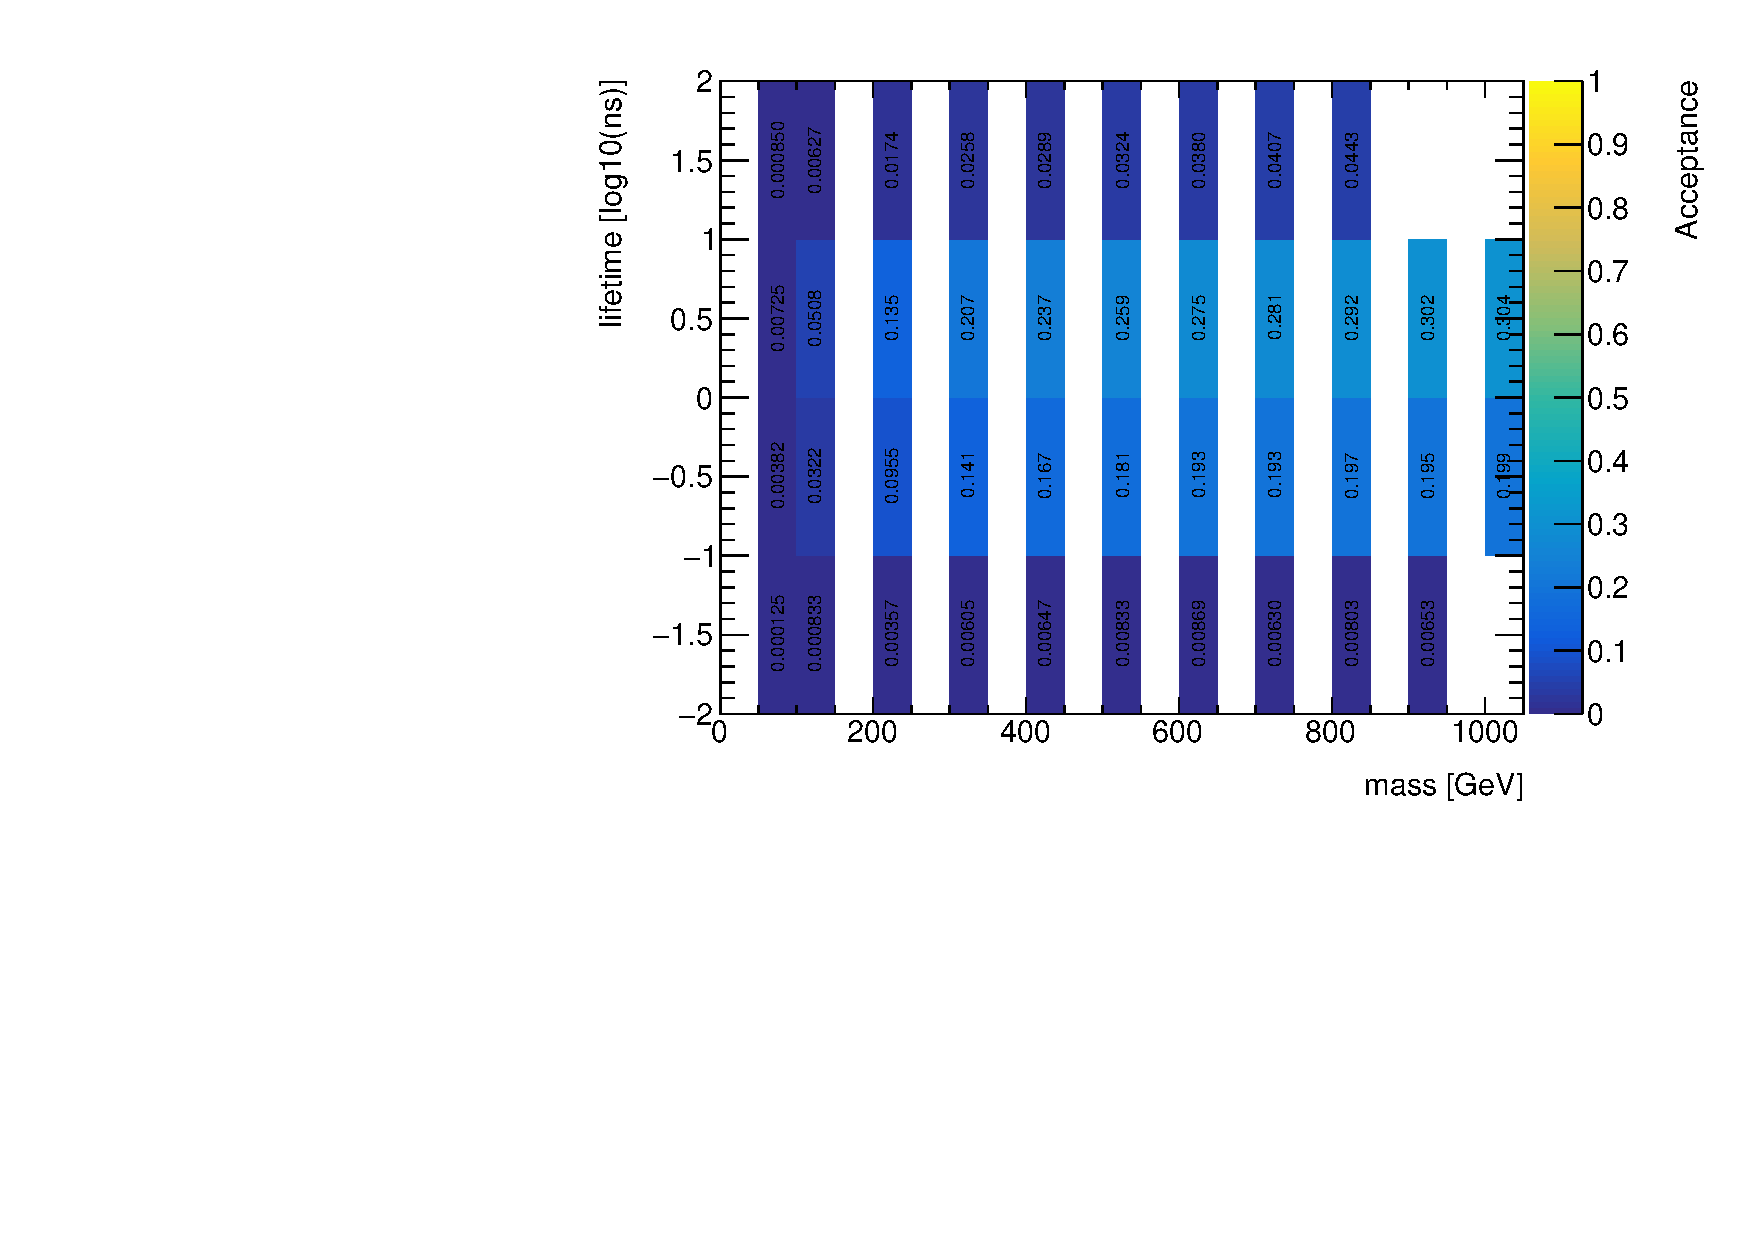
\includegraphics[width=.48\textwidth]{figures/event_selection/mm_slep_acc.pdf}
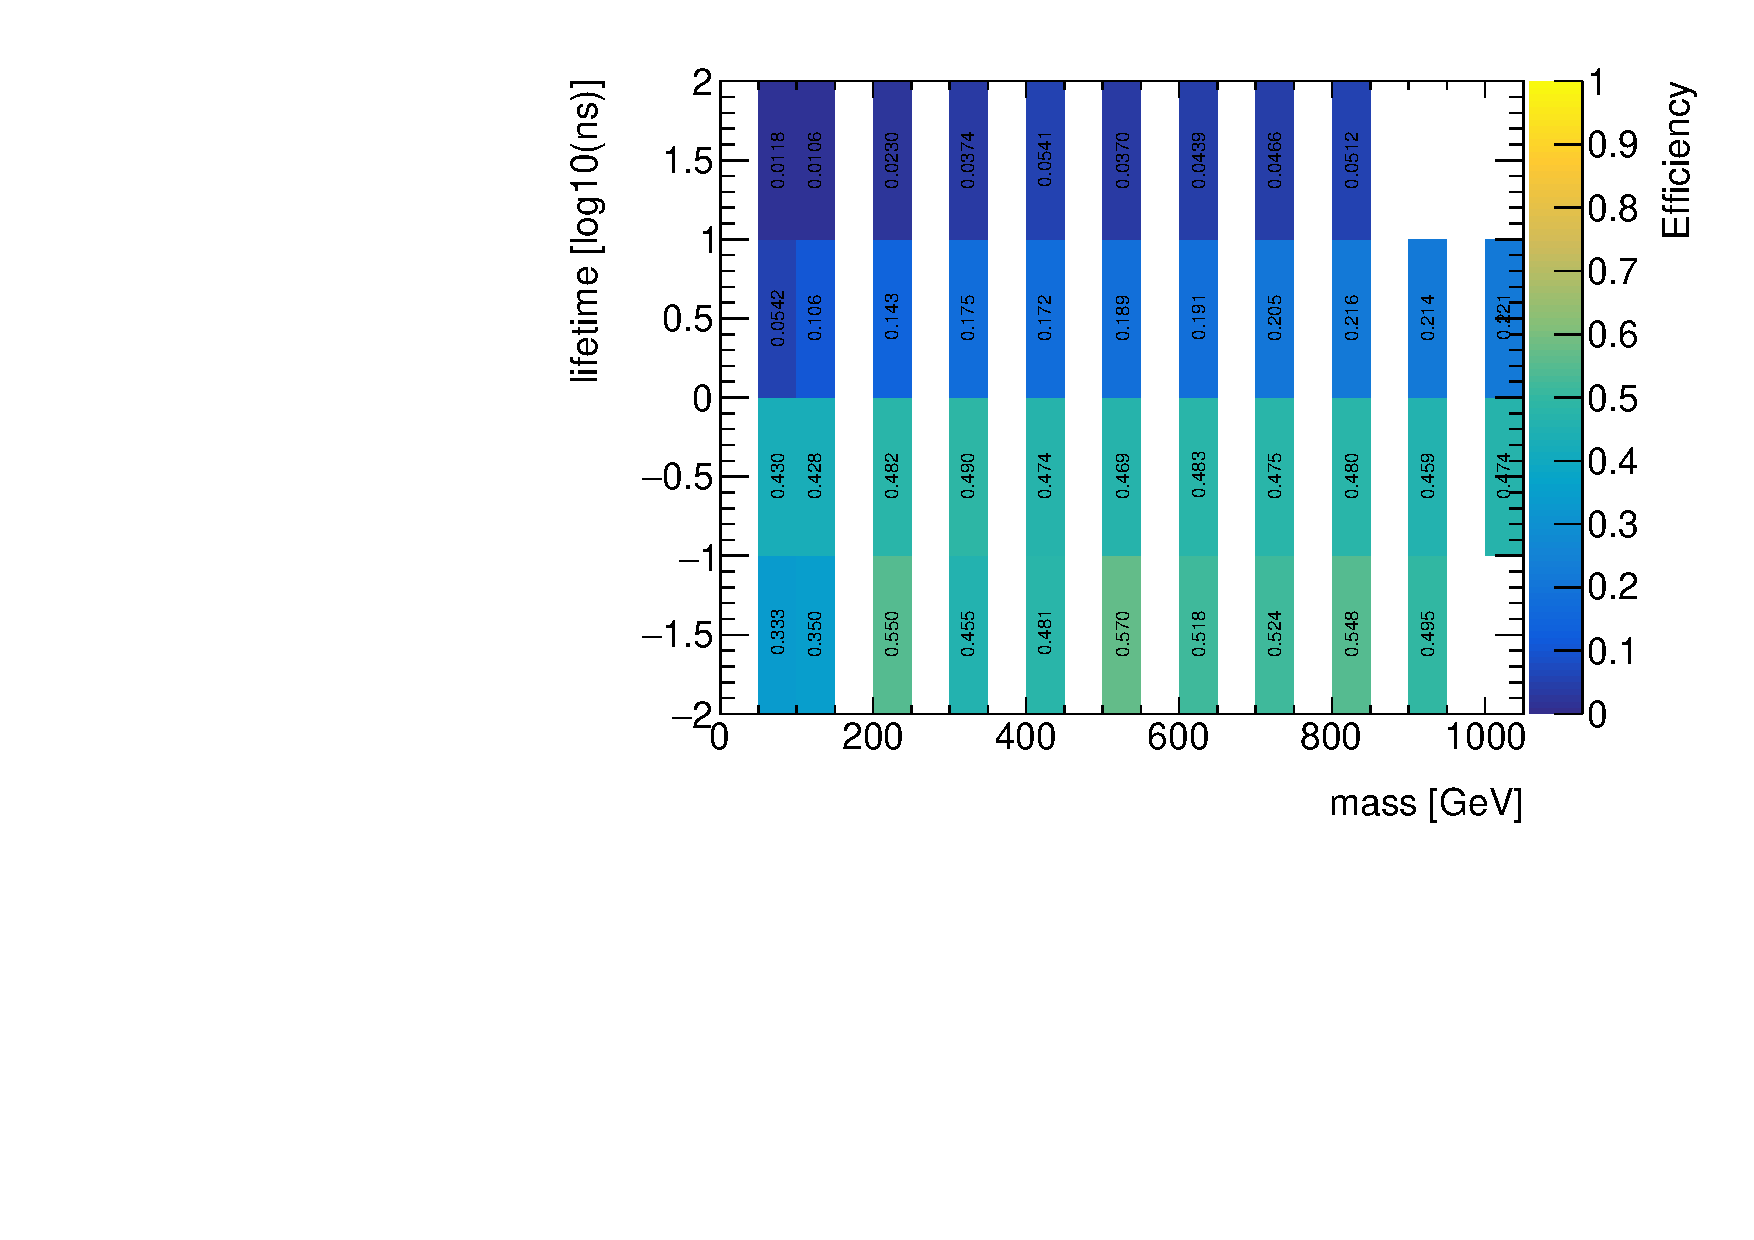
\includegraphics[width=.48\textwidth]{figures/event_selection/mm_slep_eff.pdf}
\caption{Acceptance (left) and efficiency for \smu decaying to muons in SR-$\mu\mu$. The x-axis shows the possible masses of the \smu and the y-axis its possible lifetime.}
\label{fig:acc-eff-mm}
\end{figure}

\begin{figure}[htbp]
\centering
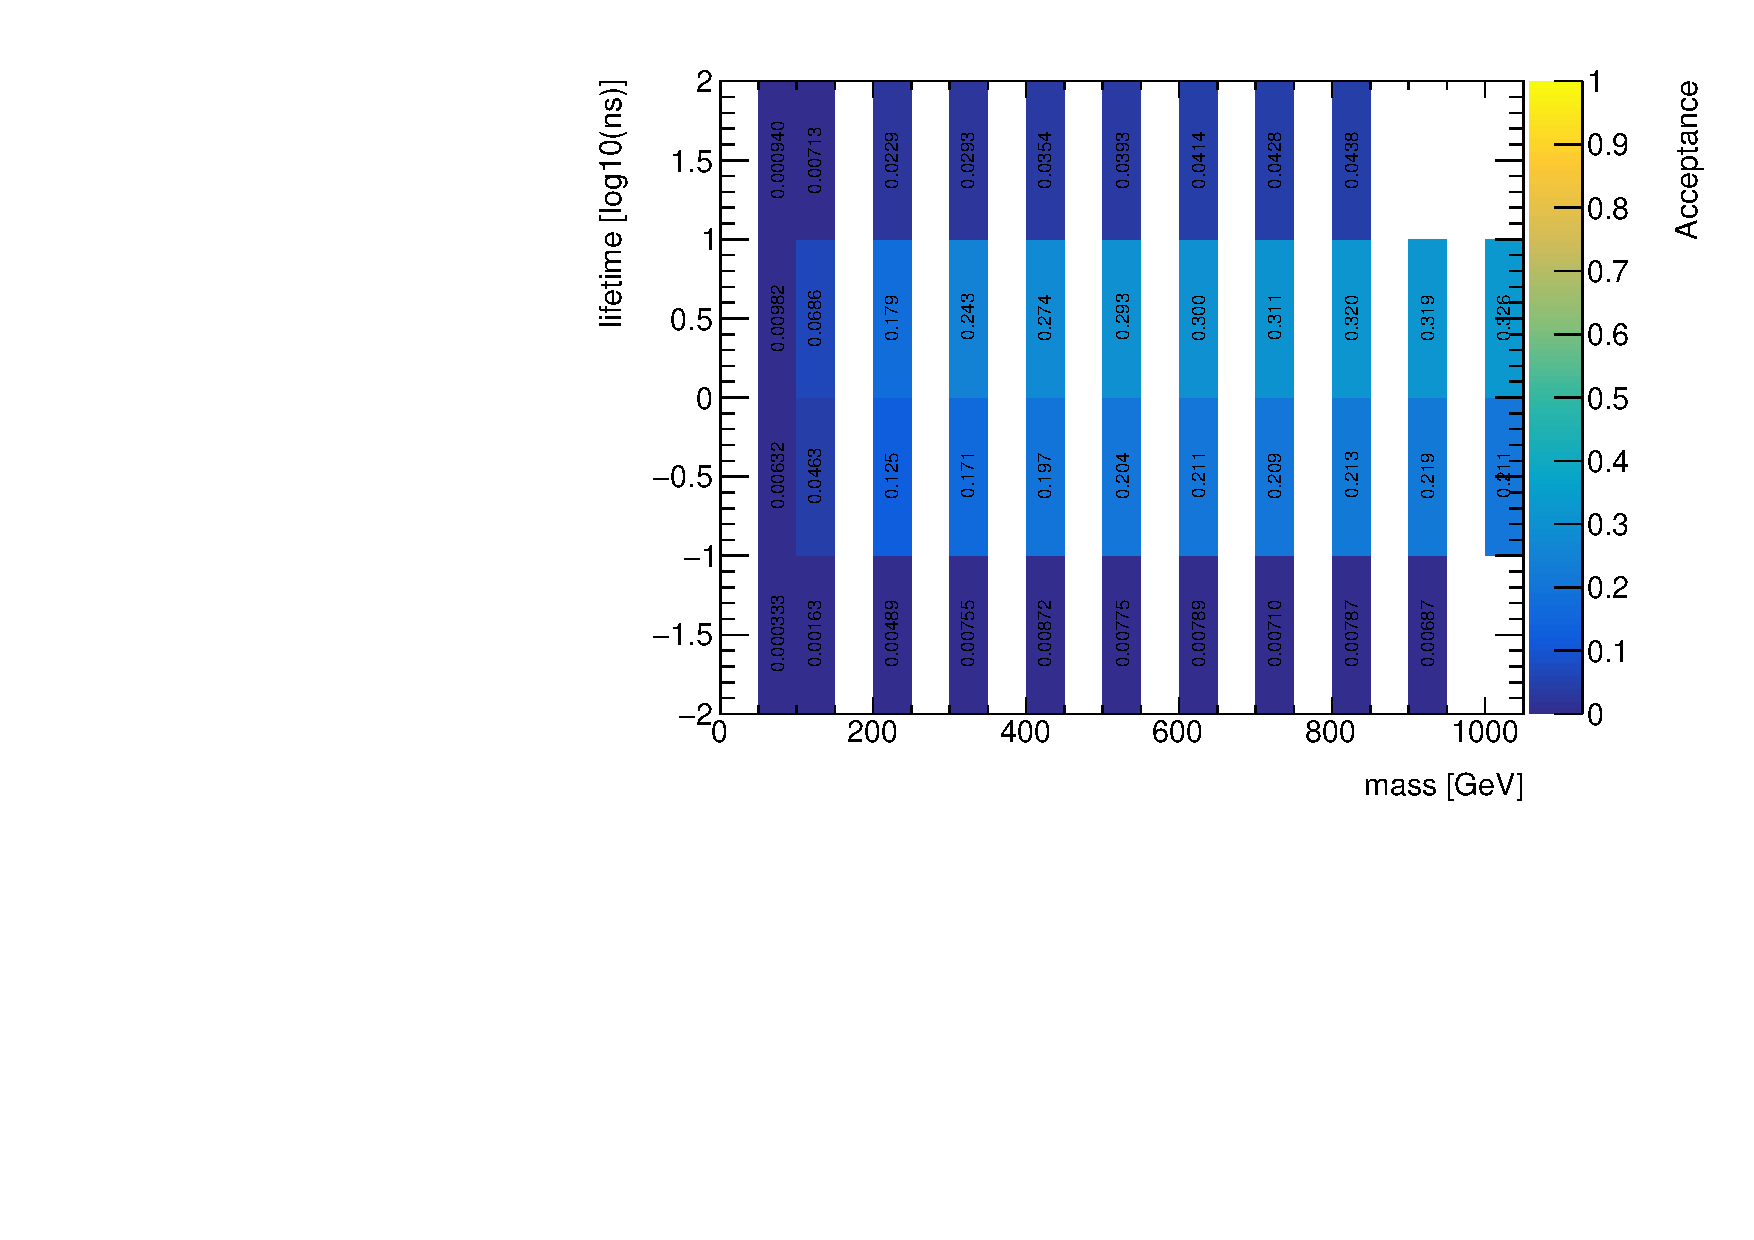
\includegraphics[width=.48\textwidth]{figures/event_selection/ee_slep_acc.pdf}
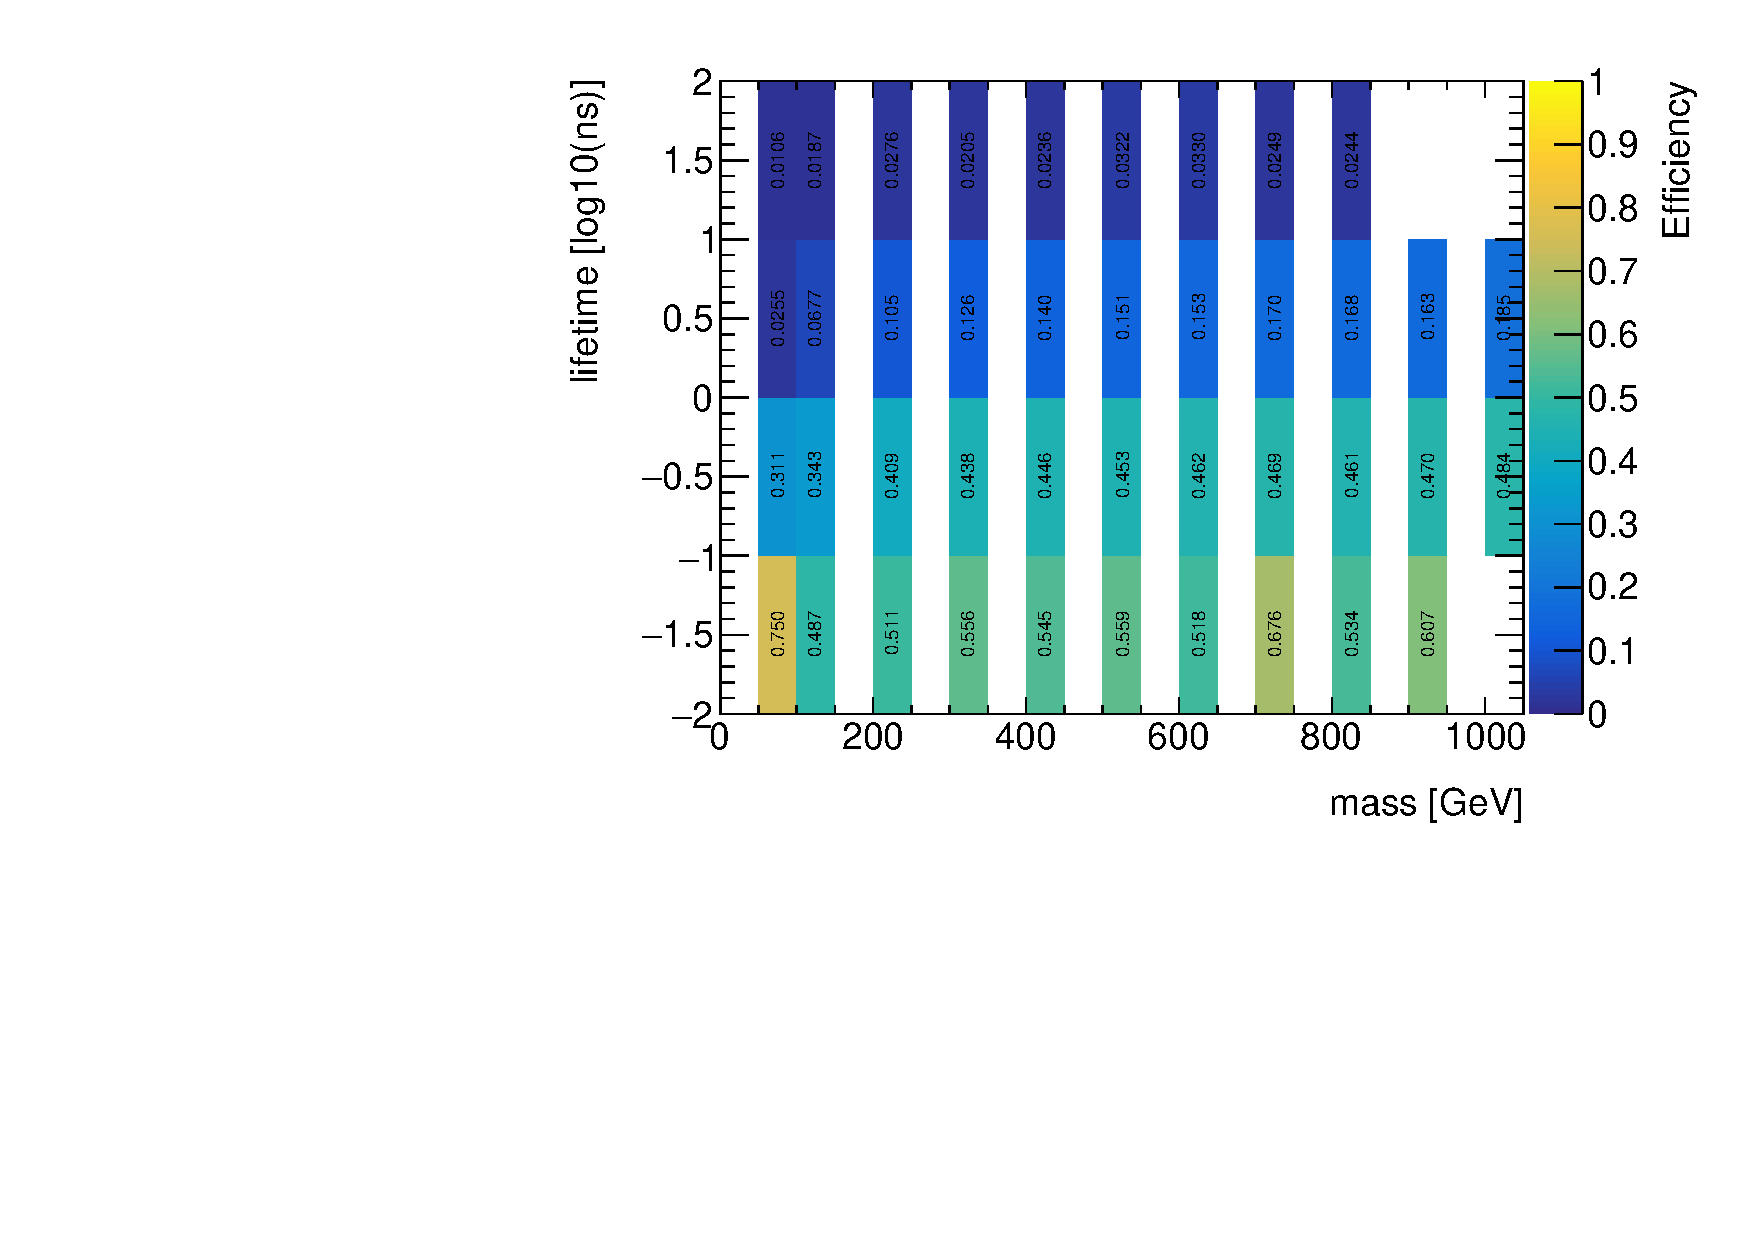
\includegraphics[width=.48\textwidth]{figures/event_selection/ee_slep_eff.pdf}
\caption{Acceptance (left) and efficiency for \selec decaying to electrons in SR-$ee$. The x-axis shows the possible masses of the \selec and the y-axis its possible lifetime.}
\label{fig:acc-eff-ee}
\end{figure}

\begin{figure}[htbp]
\centering
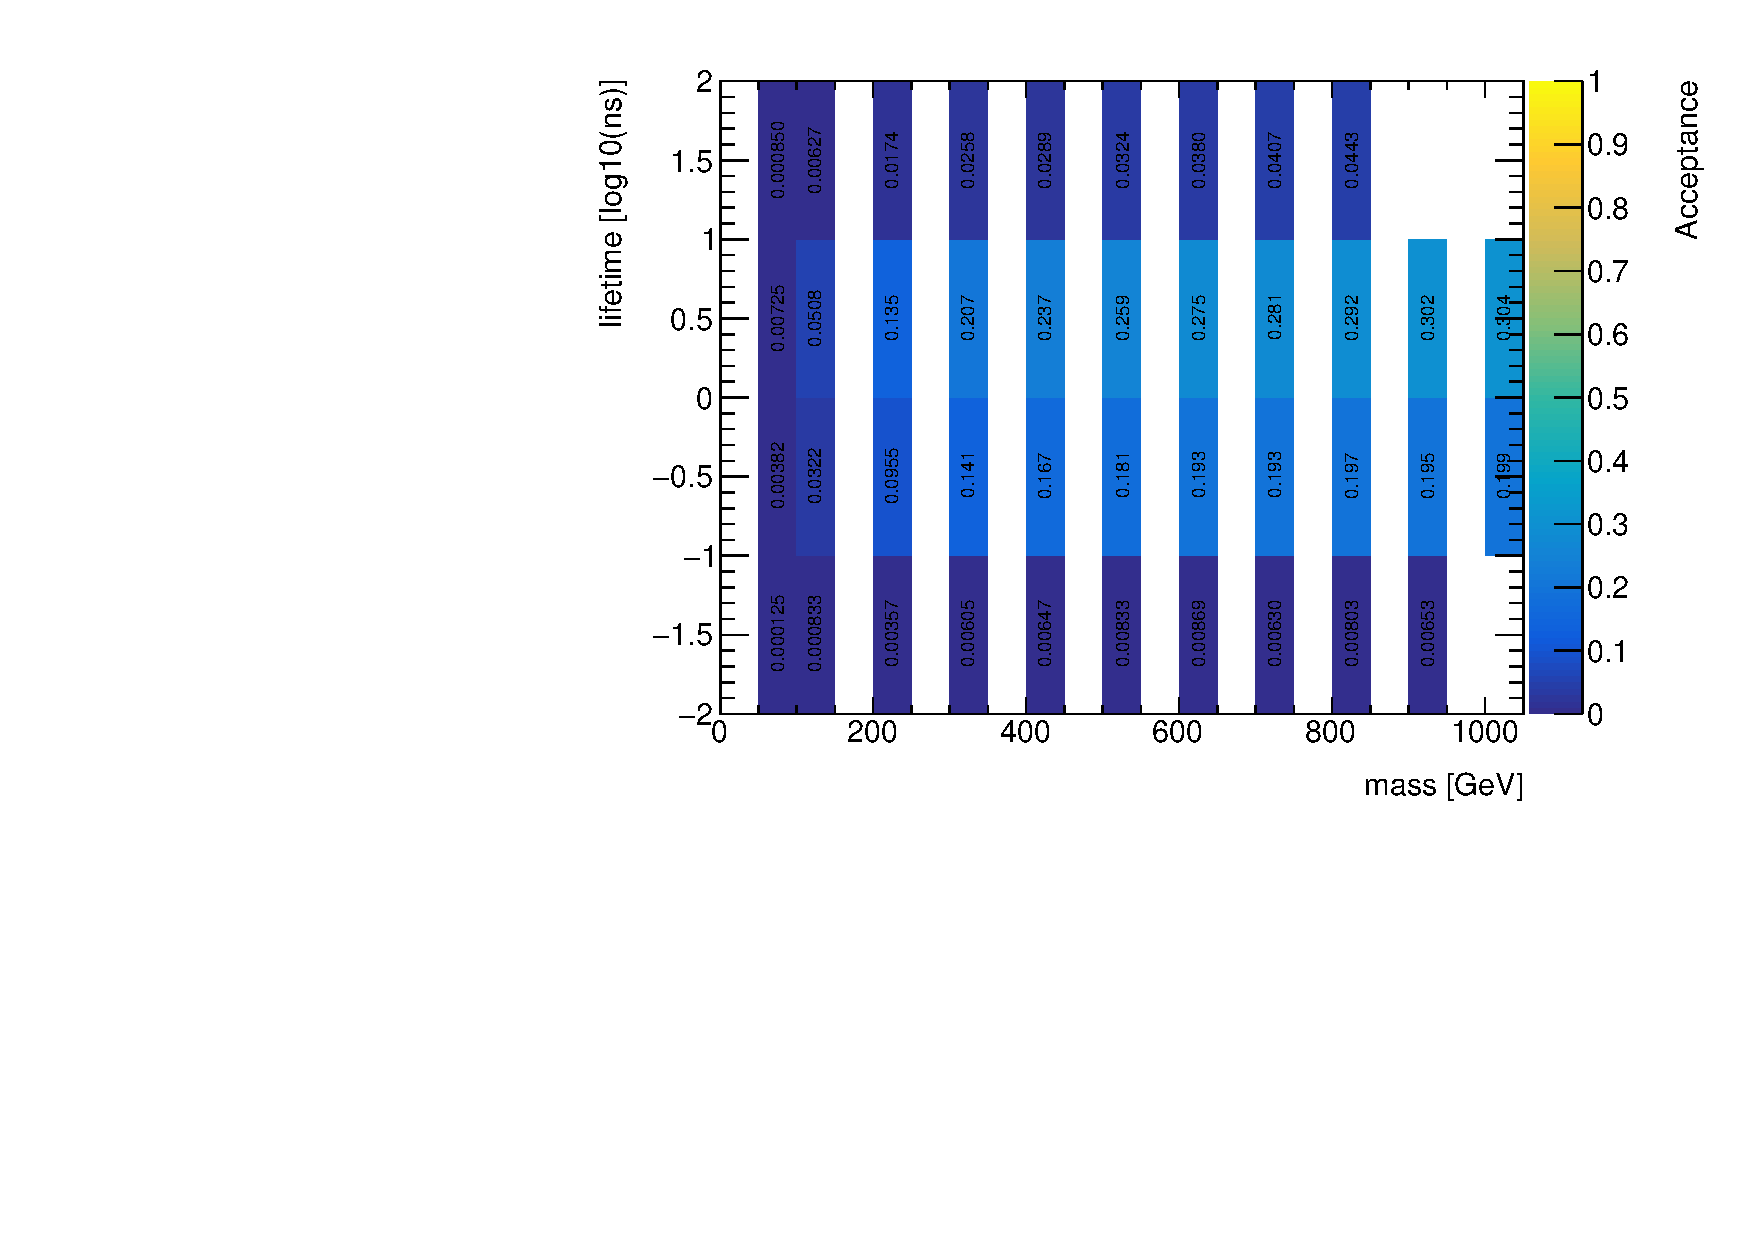
\includegraphics[width=.48\textwidth]{figures/event_selection/mm_slep_acc.pdf}
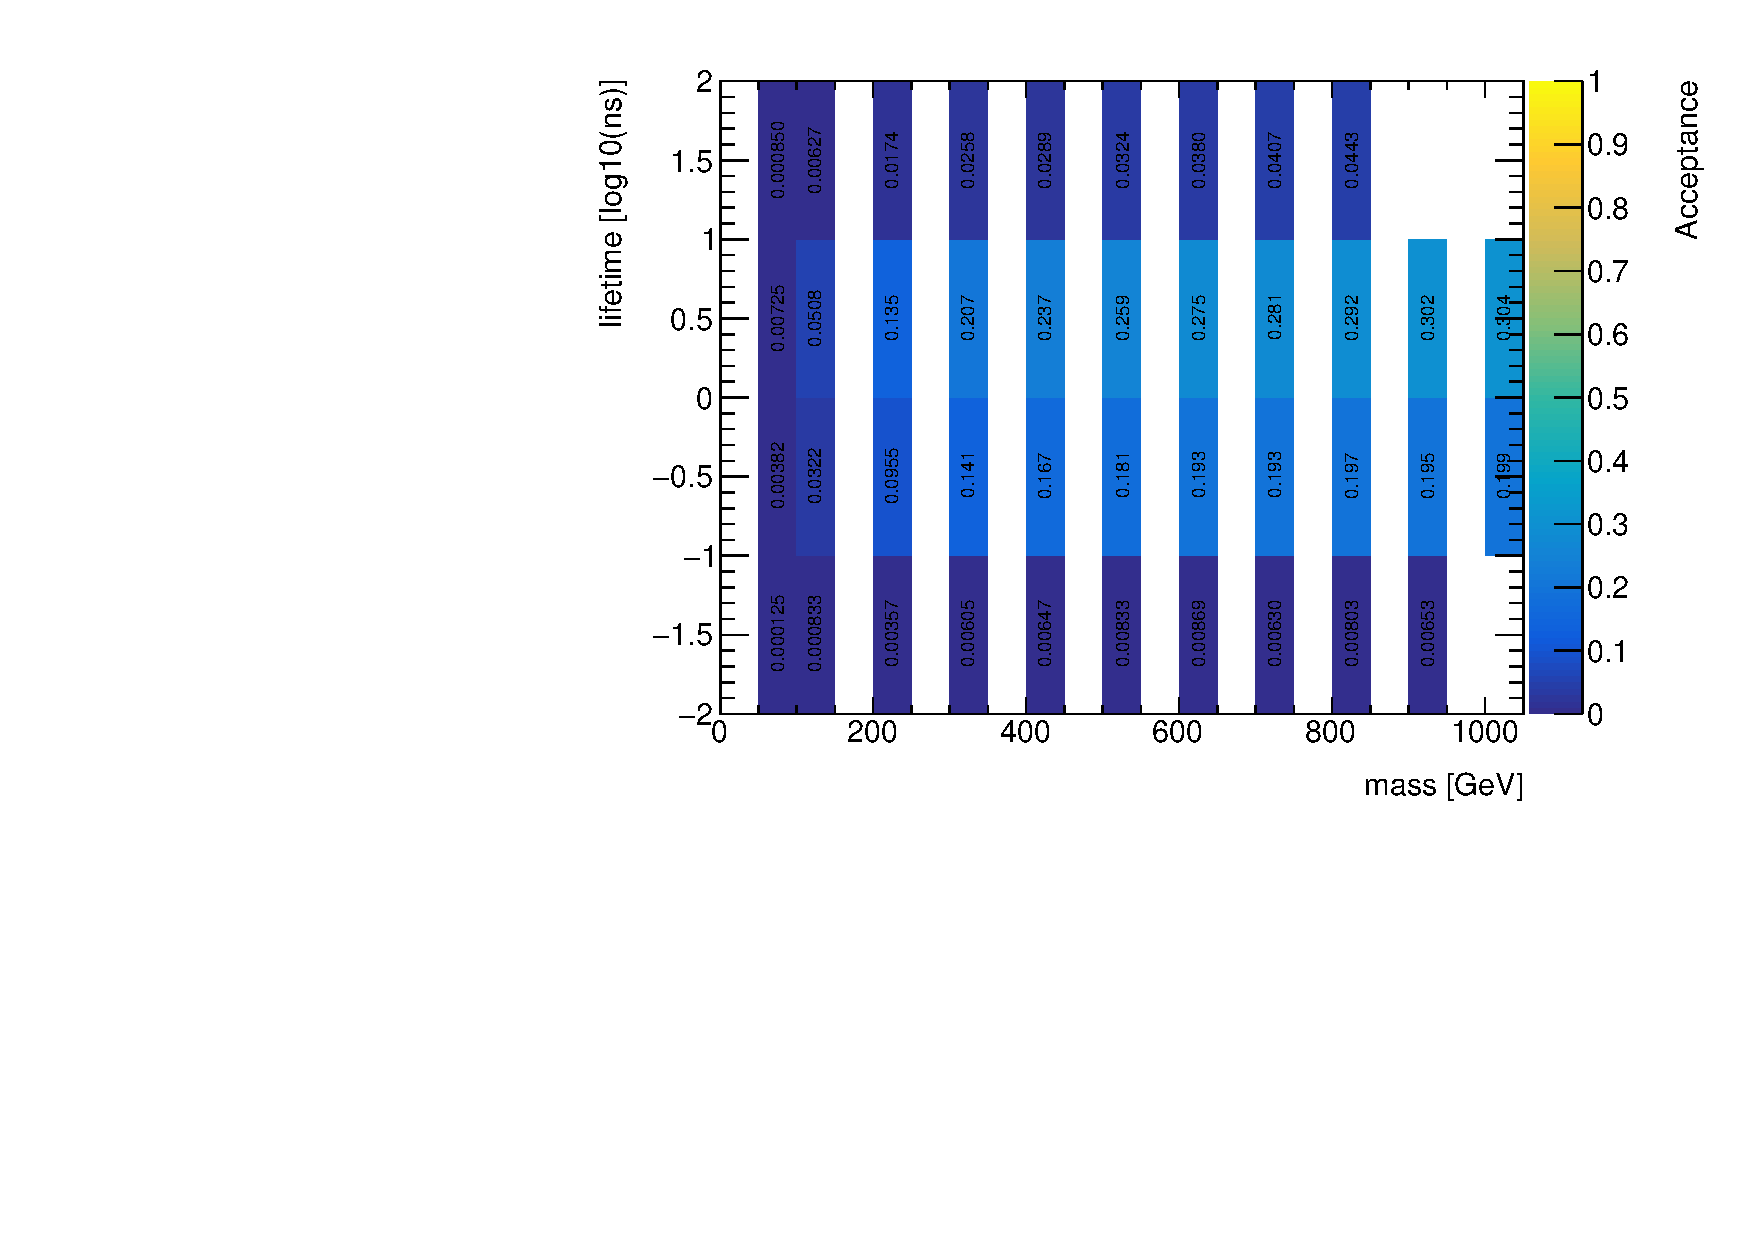
\includegraphics[width=.48\textwidth]{figures/event_selection/mm_slep_acc.pdf}
\caption{Acceptance (left) and efficiency for \stau s decaying to taus in SR-$\mu\mu$, SR-$ee$, and SR-$e\mu$ combined. The x-axis shows the possible masses of the stau and the y-axis its possible lifetime.}
\label{fig:acc-eff-em}
\end{figure}




